\documentclass{article}
\usepackage{pythonhighlight}
\usepackage{graphicx}
\usepackage{ctex}
\usepackage[left=3cm,top=3cm,right=3cm]{geometry}
\usepackage{hyperref}
% TITLE PAGE CONTENT %%%%%%%%%%%%%%%%%%%%%%%%
%%%%%%%%%%%%%%%%%%%%%%%%%%%%%%%%%%%%%%%%%%%%%
\newcommand{\labno}{09}
\newcommand{\labtitle}{EE208 Hadoop Streaming}
\newcommand{\authorname}{周李韬}
\newcommand{\studentno}{518030910407}
\newcommand{\classno}{F1803016}
% END TITLE PAGE CONTENT %%%%%%%%%%%%%%%%%%%%


\begin{document}

\begin{center}
{\LARGE \textsc{Laboratory No. \labno:} \\ \vspace{4pt}}
{\Large \textsc{\labtitle} \\ \vspace{4pt}} 
\rule[13pt]{\textwidth}{1pt} \\ \vspace{15pt}
{\large By: \authorname \\ \vspace{10pt}
No. \studentno \\ \vspace{10pt}
SJTU \classno \\ \vspace{10pt}
\today \vspace{20pt}}
\end{center}



\section{实验准备}

\subsection{实验环境}
\begin{itemize}
\item\textbf{Environment} Ubuntu 16.04 (on Virtual Machine)
\item\textbf{Tools} Hadoop 2.7.3, openjdk-8-jdk
\end{itemize}

\subsection{实验目的}

本实验中,我们需要借助Hadoop中的Map-Reduce模型,实现分布式地计算文章中单词平均长度,计算一张图中的PageRank。

\subsection{实验原理}

Map-Reduce的原理在上一次实验中已阐述。简单来说,Map对输入数据进行运算后,会产生一系列中间变量,随后Reduce函数对中间变量进行运算,得到输出结果。其中,Map和Reduce过程需要能够实现分布式运算。在Hadoop的MapReduce模型中,在Map和Reduce之间,会有一次对数据的排序过程,利用这一功能,Map结果将会按照数据的Key排序,从而使下一步Reduce提供帮助。

\paragraph{计算单词平均长度}



\paragraph{计算PageRank}
本实验中,我们假设图是以邻接表的形式存储在文本文件中的,



\section{实验步骤}

\subsection{安装Hadoop}

根据实验材料中的提示,我们在Linux虚拟机中为分配了账户,依次下载、安装了java8,Hadoop2.7.3,并完成了Hadoop的配置。

\subsection{计算$\pi$}

Hadoop计算$\pi$的原理已在上一节中进行解释。Hadoop Example中已对改运算进行了封装,我们调用时需要传入两个参数,map是运行map任务的个数,sample是每个map任务中取样的个数。map与sample之积就是一次统计中的全部试验个数。我们在命令行中调用该函数的命令如下。
\begin{python}
hadoopjar /usr/local/hadoop/share/hadoop/mapreduce/hadoop-mapreduce-examples-2.7.3.jar pi 2 10
\end{python}

试验结果如下所示:
\begin{table}[htbp]
\begin{tabular}{cccccc}
\hline
\textbf{Experiment} & \textbf{\begin{tabular}[c]{@{}c@{}}Number of\\ Maps\end{tabular}} & \textbf{\begin{tabular}[c]{@{}c@{}}Number of\\ Samples\end{tabular}} & \textbf{\begin{tabular}[c]{@{}c@{}}Total Sample\\ Counts\end{tabular}} & \textbf{\begin{tabular}[c]{@{}c@{}}Running\\ Time(s)\end{tabular}} & \textbf{\begin{tabular}[c]{@{}c@{}}Estimated\\ pi\end{tabular}} \\ \hline
1                   & 2                                                                 & 10                                                                   & 20                                                                     & 18.275                                                             & 3.8                                                             \\
2                   & 5                                                                 & 10                                                                   & 50                                                                     & 22.300                                                             & 3.28                                                            \\
3                   & 1                                                                 & 100                                                                  & 100                                                                    & 17.244                                                             & 3.2                                                             \\
4                   & 10                                                                & 10                                                                   & 100                                                                    & 26.427                                                             & 3.2                                                             \\
5                   & 2                                                                 & 100                                                                  & 200                                                                    & 17.759                                                             & 3.12                                                            \\
6                   & 10                                                                & 100                                                                  & 1000                                                                   & 27.978                                                             & 3.148                                                           \\
7                   & 20                                                                & 100000                                                               & 2000000                                                                & 48.594                                                             & 3.141504                                                        \\
8                   & 100                                                               & 100000                                                               & 10000000                                                               & 75.672                                                             & 3.1415844                                                       \\
9                   & 10                                                                & 1000000                                                              & 10000000                                                               & 27.616                                                             & 3.1415844                                                       \\
10                  & 10                                                                & 10000000                                                             & 100000000                                                              & 27.340                                                             & 3.14159256                                                      \\ \hline
\end{tabular}
\end{table}

从相同样本数的实验中可以得知,在不改变随机数列的种子的情况下,该样例的算法是确定性的。比较3、4实验可得,在数据量较小的情况下,Maps过多会增加运行时间,比较8、9实验可得,过多的Maps在超过本机运行能力的情况下,也会拖慢运行时间,比较9、10实验则可得,在选取合适的Maps条件下,分布式计算能够有效减小甚至消除由于样本数增多而造成的时间消耗。根据实验结果所得,当样本数达到$10^8$数量级时,$\pi$的估算能够达到5位小数的精度。


\begin{figure}[htbp]
\centering
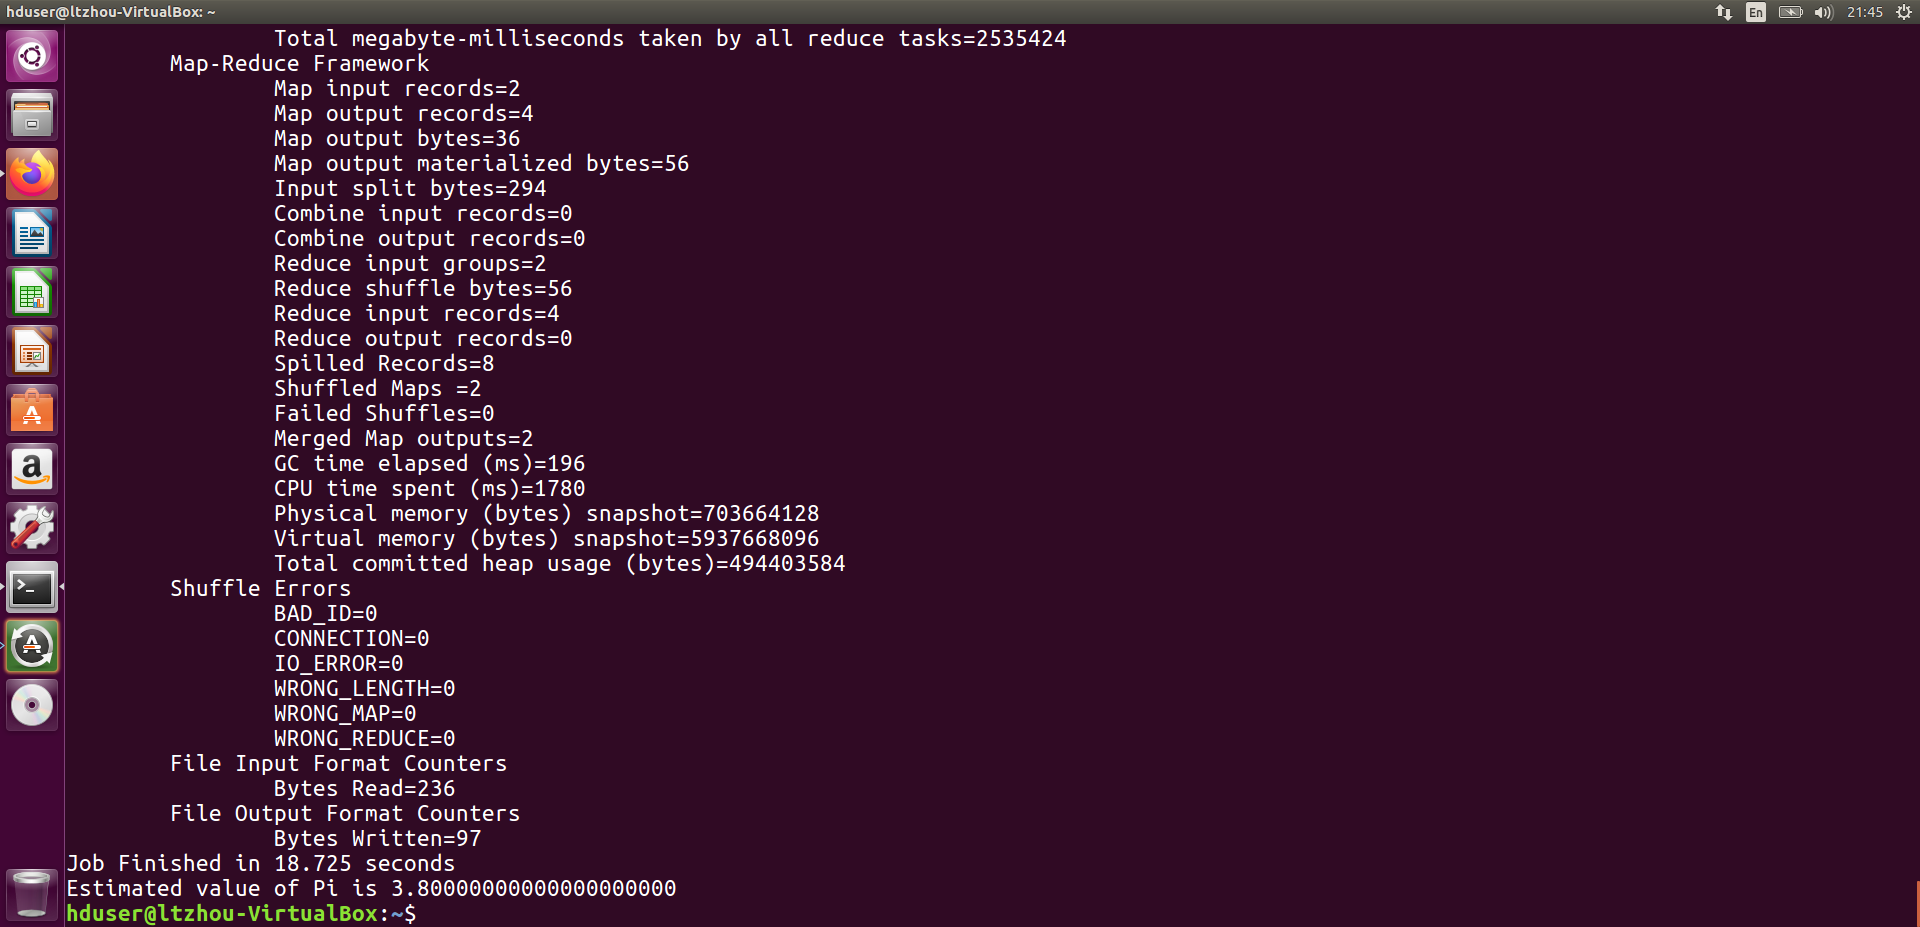
\includegraphics[width=13.5cm]{img/2-10.png}
\caption{Map=2, Sample=10时运行结果实例}
\label{fig:2-10}
\end{figure}

\begin{figure}[htbp]
\centering
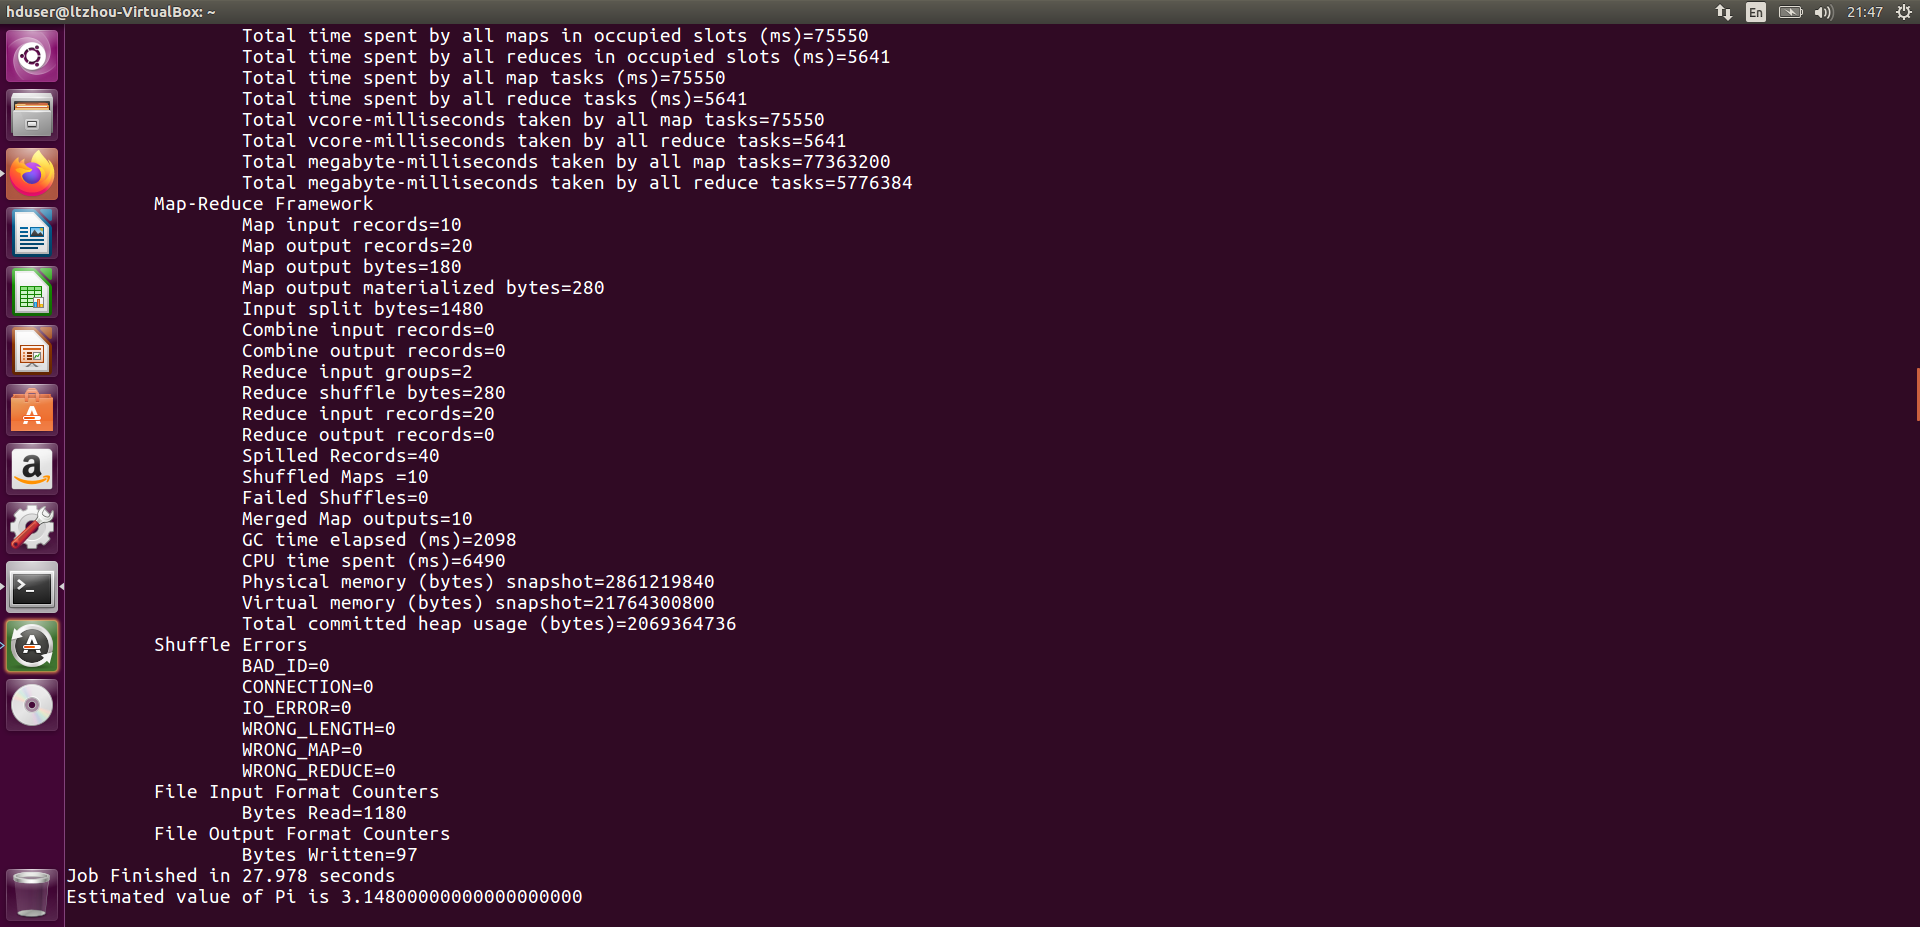
\includegraphics[width=13.5cm]{img/10-100.png}
\caption{Map=10, Sample=100时运行结果实例}
\label{fig:2-10}
\end{figure}



\section{实验总结}
\paragraph{概述}
本实验中,我们完成了Hadoop的安装、配置,并通过实验分布式地计算了$\pi$的估计值。

\paragraph{感想}
通过本次实验的学习,我体会到到了分布式运算带来的运算效率提升。分布式运算能够帮助我们更充分地利用、扩展现有的硬件资源,带来性能的提升。我也通过实验的尝试,学习了MAP-REDUCE模型的思想,希望这次实验的学习能够为以后的LAB做好铺垫。


\end{document}

